\section{Introduction}

\begingroup
\begin{figure}[!ht]
  \centering
  \subfigure[]{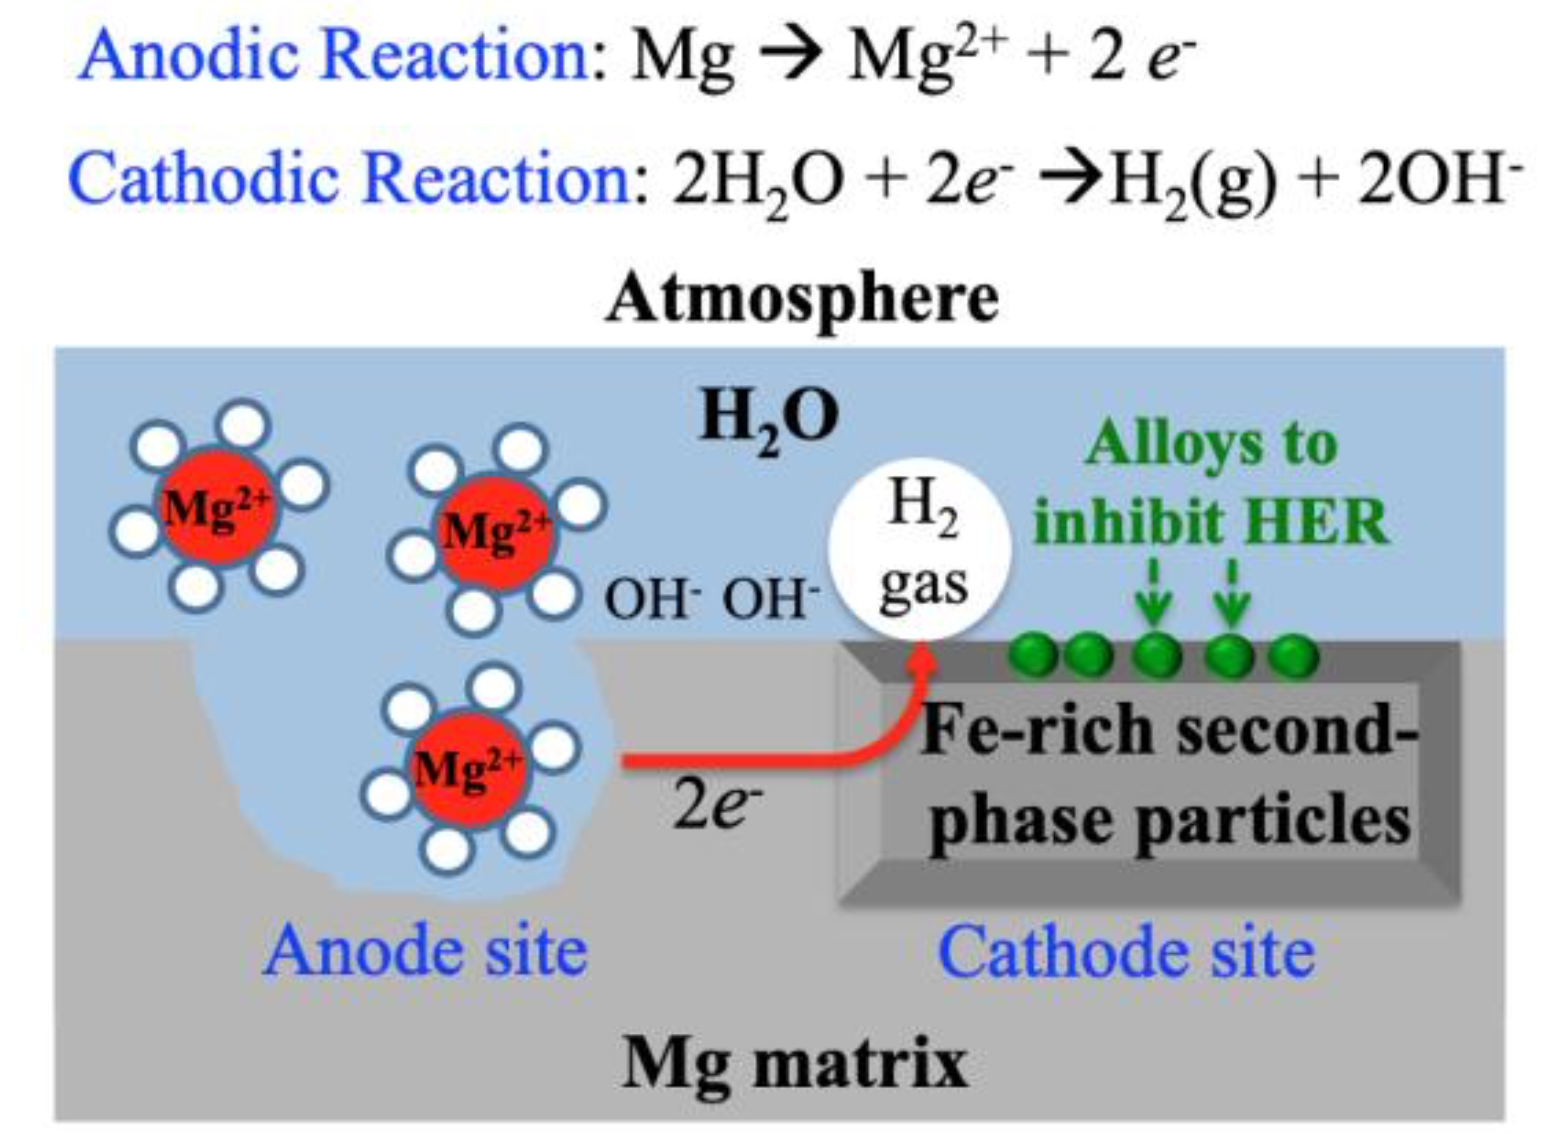
\includegraphics[width=0.49\linewidth]{Chap3/plots/Fig1a.png}}\label{Chap:Mg_H:fig:1a}
  \subfigure[]{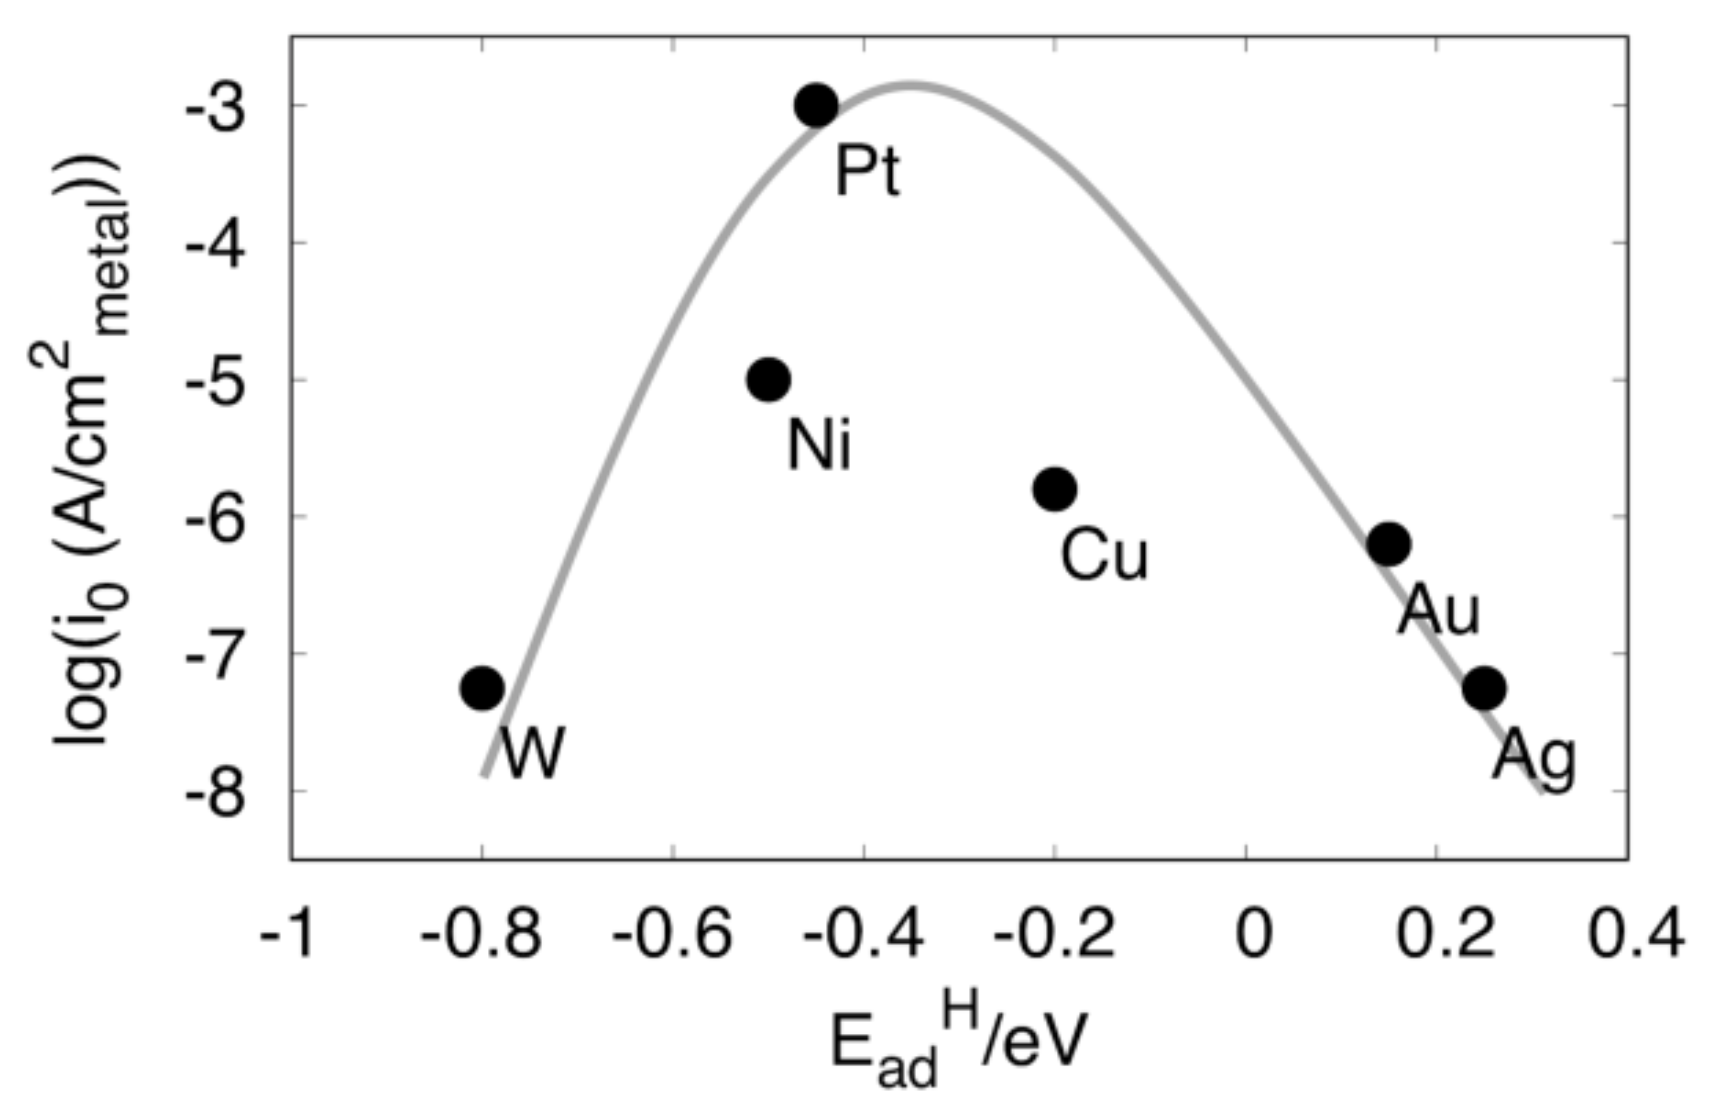
\includegraphics[width=0.49\linewidth]{Chap3/plots/Fig1b.png}}\label{Chap:Mg_H:fig:1b}
\caption[Illustration of corrosion reaction mechanism on Mg and the alloying strategy to inhibit \ac{HER}]{(a) Illustration of corrosion reaction mechanism on Mg and the alloying strategy to inhibit the \ac{HER} as the cathodic reaction. The anodic reaction occurs to Mg matrix by dissolving one Mg atom to produce a $Mg^{2+}$ cation into the electrolyte and two electrons for HER as the cathodic reaction, which occurs on surfaces of second-phase particles, usually rich in Fe and other transition metal elements, to produce a $\text{H}_\text{2}$ gas molecule. A possible strategy to reduce \ac{HER} rate is to change the H adsorption energy on the surfaces of second-phase particles by proper alloying. (b) Exchange current density of \ac{HER}, $\log(i_0(A/cm^2_{metal})])$, measured in experiments under pH$=$12 vs. H adsorption energy $E_{ad}^H$ defined by Eq. \ref{Chap:Mg_H:eq:H_ads} from \ac{DFT} calculations. This figure is adapted from the data of Sheng et al.\cite{sheng2013correlating}. A higher exchange current density corresponds to a faster \ac{HER} and a higher corrosion rate. The volcano-shaped solid curve line is plotted only for an illustration the relation between $\log(i_0)$ and $E_{ad}^H$ without quantitative accuracy.}
  \label{Chap:Mg_H:fig1}
\end{figure}
\endgroup

Magnesium alloys are potential candidates for lightweight structural components in transportation industries and other applications due to their low density and high specific strength. Substantial effort has been focused on exploring cast and wrought magnesium (Mg) alloys for application in vehicle propulsion systems and body structures, for example, as part of light-weighting strategies \cite{luo2005development, luo2006wrought,carter2011structural, jekl2015development, luo2013magnesium}. However, corrosion in aqueous and atmospheric environments is one of two significant challenges facing a broader implementation of current Mg alloys in vehicles. The other challenge is poor room temperature formability of Mg sheet alloys in stamping, a consequence of the anisotropy in plasticity response associated with the various dislocation slip systems in the \ac{HCP} structure \cite{yasi2010first}. Post-forming surface treatments can be applied to mitigate Mg corrosion \cite{zheng2005corrosion}.
In an aqueous environment, the coupling between regions of anodic dissolution of Mg and cathodic reduction of water drives galvanic corrosion leading to the removal of Mg and the formation of pits surrounding second-phase particles as cathode sites \cite{birbilis2014evidence, zeng2006review}. Magnesium has a highly negative standard electrode potential of -2.37 V relative to the \ac{SHE}, making it a very active anode (all electrode potential values are relative to the \ac{SHE} in this paper). Anodic dissolution of Mg via
\begin{align}
Mg \rightarrow Mg^{2+} + 2e^{-}
 \label{Chap:Mg_H:eq:anodic_dissolution}
\end{align}
couples with the cathodic reaction, which is the reduction of water in an alkaline electrolyte
\begin{align}
2H_2O + 2e^{-} \rightarrow H_{2}(g) + 2OH^{-}
 \label{Chap:Mg_H:eq:cathodic_reaction}
\end{align}
Eq. \ref{Chap:Mg_H:eq:cathodic_reaction} is the \ac{HER} with a standard electrode potential of -0.828 V relative to \ac{SHE}. The overall reaction mechanism is illustrated in Fig. \ref{Chap:Mg_H:fig1} (a).

Corrosion on Mg proceeds without any limitation for pH < 11 since oxygen is not involved and no passivating surface layer forms \cite{liu2016controlling,ralston2012effect}. Previously, it was found that Fe, Cu, Co, and Ni accelerate Mg corrosion in aqueous environments containing chlorides \cite{hanawalt1942corrosion, mcnulty1942some}. Even though Fe (an impurity often introduced during alloy processing \cite{yang2015corrosion, scharf2007iron}) has a very low solubility limit in Mg \cite{mcnulty1942some}, Fe particles in \ac{BCC} structure have been identified as cathode sites. This was demonstrated by Taub et al. \cite{taub2002mechanism} with experiments involving powdered Mg and Fe in chloride solutions. The cathodic reaction in Mg alloys typically occurs at submicron and micron-scale Fe (and Fe-rich) second-phase particles positioned at the metal-aqueous solution interface \cite{yang2015corrosion, eaves2012inhibition}. The detailed roles of Fe-rich particles as cathodic reaction sites can vary according to corrosion potentials (such as the \ac{NDE}) and the populations/sizes of Fe-rich particles \cite{hoche2016effect, yang2018effect}; the cathodic reaction rates should also depend on the surface configurations of Mg, which typically contain mixtures of porous Mg hydroxides and oxides (e.g. aluminum oxide). Hence, the accurate locations of Fe-rich particles relative to these mixtures can result in changes in corrosion rates \cite{taheri2012analysis, taheri2014towards}. Song and Atrens provided an overview of galvanic as well as other corrosion mechanisms of Mg with some useful insights \cite{song2003understanding}. Esmaily et al. presented a comprehensive summary of the recent progress of studies in Mg-alloy corrosion \cite{esmaily2017fundamentals}.

There is significant interest in designing Mg alloys that have a “built-in” corrosion inhibition mechanism \cite{eaves2012inhibition}. A possible strategy is to slow down the HER rates on cathode sites such as Fe particles in \ac{BCC} phase. The HER can be completed through either the Volmer-Heyrovsky mechanism or the Volmer-Tafel mechanism \cite{ghali2010corrosion,walling1968electrochemical}. The associated reactions are
\begin{subequations}
\begin{align}
&\text{Volmer reaction:    } & H_2O + e^- & \rightarrow H^* + OH^-
 \label{Chap:Mg_H:eq:Volmer}\\
&\text{Heyrovsky reaction:    } & H^* + H_2O + e^- & \rightarrow H_2(g) + OH^-
 \label{Chap:Mg_H:eq:Heyrovsky}\\
&\text{Tafer reaction:    }
& 2H^* & \rightarrow H_2(g)
 \label{Chap:Mg_H:eq:Tafel}
\end{align}
\end{subequations}
Here * means the corresponding atom/molecule is adsorbed on cathode surface sites. The Volmer-Heyrovsky mechanism proceeds first via Eq. \ref{Chap:Mg_H:eq:Volmer} followed by Eq. \ref{Chap:Mg_H:eq:Heyrovsky}. The Volmer-Tafel mechanism involves Eq. \ref{Chap:Mg_H:eq:Volmer} twice followed by Eq. \ref{Chap:Mg_H:eq:Tafel}. The equilibrium potentials of Eqs. \ref{Chap:Mg_H:eq:Volmer}, \ref{Chap:Mg_H:eq:Heyrovsky} and \ref{Chap:Mg_H:eq:Tafel} depend on the free energies of hydrogen atoms adsorbed on cathode surface sites.


The slowing down of the HER as the cathodic reaction requires the reduction of reaction rates via the Volmer-Heyrovsky mechanism and the Volmer-Tafel mechanism. Regarding the Volmer reaction in Eq. \ref{Chap:Mg_H:eq:Volmer}, its fast kinetics favors the strong adsorption of an H atom on a cathode surface site to increase its thermodynamic driving force since H* is its reaction product. However, the fast kinetics of the Heyrovsky and Tafel reactions in Eq. \ref{Chap:Mg_H:eq:Heyrovsky} and \ref{Chap:Mg_H:eq:Tafel}, respectively, require the weak adsorption of an H atom since H* is the reactant on the left side of each equation. Thus, the adsorption strength of H atoms on a cathode surface must be at an intermediate-range to reach the maximum \ac{HER} rate: this is the Sabatier principle \cite{medford2015sabatier}. Fig. \ref{Chap:Mg_H:fig1} (b) shows the exchange-current density of the \ac{HER} vs. H adsorption energy, $E_{ad}^H$, in alkaline electrolytes \cite{sheng2013correlating}: the highest values of $\log(i_0)$ corresponding to the fastest \ac{HER} rate appear for the intermediate $E_{ad}^H$. Similar plots of \ac{HER} rate in acid electrolyte vs. $E_{ad}^H$ have been explored on different metals, even though the detailed reaction mechanisms in the \ac{HER} differ from those in an acid electrolyte. Therefore, to slow down the overall \ac{HER} rate on cathode sites, either the adsorption strength of H must be strongly enhanced, so that the rate of the Heyrovsky and Tafel reactions is largely decreased, or the adsorption of H must be significantly weakened thereby reducing the rate of the Volmer reaction.

\newpage
\begingroup
\begin{figure}[!ht]
  \centering
  \subfigure[]{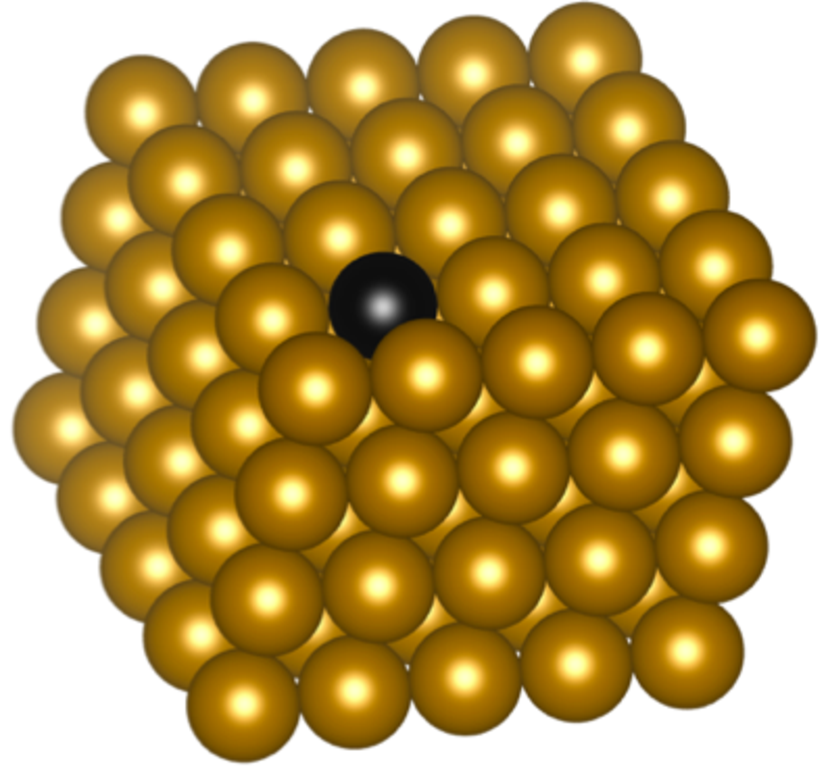
\includegraphics[width=0.45\linewidth]{Chap3/plots/Fig2a.pdf}}\label{Chap:Mg_H:fig:2a}
  \subfigure[]{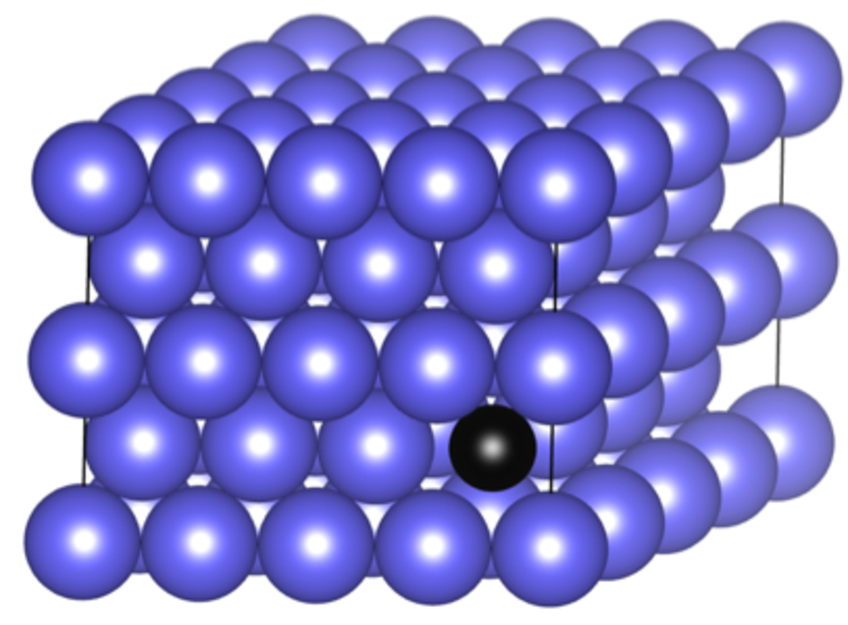
\includegraphics[width=0.45\linewidth]{Chap3/plots/Fig2b.pdf}}\label{Chap:Mg_H:fig:2b}\\
  \subfigure[]{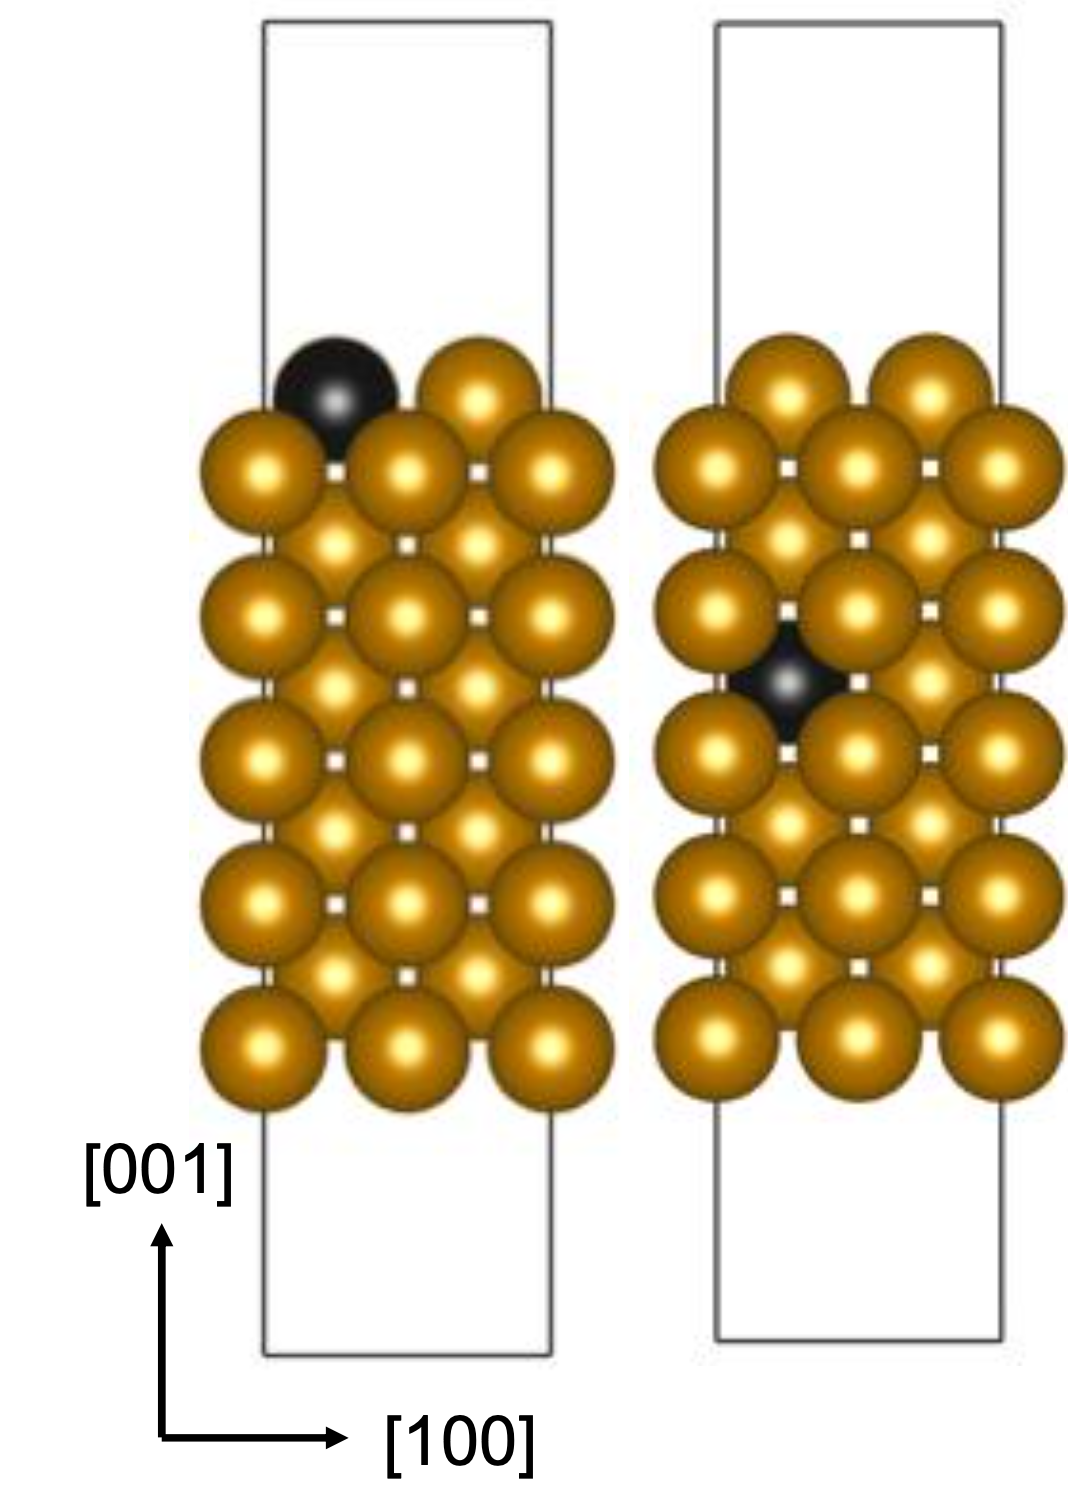
\includegraphics[width=0.42\linewidth]{Chap3/plots/Fig2c.png}}\label{Chap:Mg_H:fig:2c}
  \subfigure[]{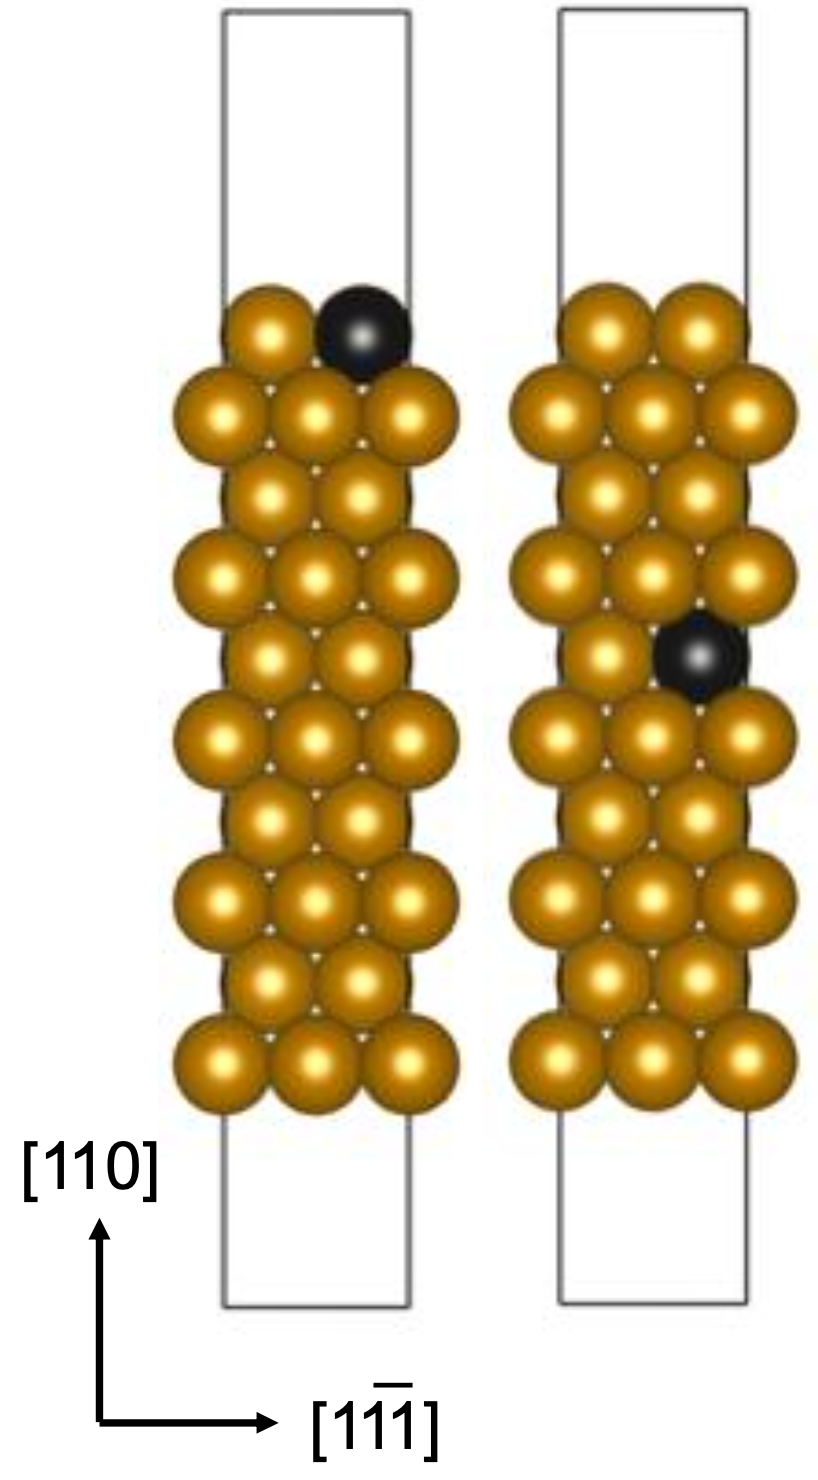
\includegraphics[width=0.32\linewidth]{Chap3/plots/Fig2d.png}}\label{Chap:Mg_H:fig:2d}
\caption[Perspective and side views of a generic alloying element in the simulation]{(a) and (b): Perspective view of a generic alloying element (black) in (a) bulk Fe (gold) and (b) bulk Mg (blue) lattice. (c)/(d): Side views of a generic alloying element (black) positioning in (2x2) Fe (100) (c) /Fe (110) (d) surface slab (the left sub-figure) at a substitutional site in the top surface layer and (the right sub-figure) at a substitutional site inside bulk Fe ($5^{th}$ layers from the top surface).}
  \label{Chap:Mg_H:fig2}
\end{figure}
\endgroup


Experimentalists have identified Arsenic (As) and Germanium (Ge) as Mg corrosion inhibitors. These are thought to exert a form of “kinetic control” over Mg corrosion, which is somewhat surprising from the standpoint that most elements tend to increase Mg corrosion rates \cite{liu2016controlling}. Eaves et al. \cite{eaves2012inhibition} were among the first to report that As is an effective corrosion inhibitor for commercially pure Mg with 280 ppm Fe in aqueous NaCl electrolyte. A subsequent report by Birbilis et al. \cite{birbilis2014evidence} proposed that As effectively ``poisons'' Mg corrosion by acting as a barrier for hydrogen intermediate (H*) recombination on surfaces of Fe particles (i.e. the cathode sites) thereby disrupting the formation of $\text{H}_2$(g) and, consequently, the \ac{HER} reaction. Noting that As is carcinogenic to humans, Liu et al. \cite{liu2016controlling,liu2018simultaneously} explored Ge and Ge-Zn metallurgically alloyed with pure Mg and found that Ge also interferes with cathode reactions. Other investigations have focused on adding rare earth elements to Mg \cite{birbilis2009corrosion,liu2009effect,shi2013corrosion}. New Mg-Li and Mg-Sn alloys were recently reported in which protective surface films form that prevent corrosion \cite{xu2015high,cain2019corrosion}. While these studies have pointed to an effect of a few elemental additives on Mg corrosion, the experimental literature has not, to our knowledge, provided a more expansive study of Mg corrosion inhibiting elements, and it is essentially silent regarding the role of electronic structure and chemical bonding at surfaces of Fe particles especially with regards to possible disruption of the \ac{HER}.


In this chapter, we use a high-throughput computational procedure based on \ac{DFT} to search for potential Mg corrosion inhibiting elements. We first search for other elements that can effectively slow down/disrupt the \ac{HER} by computing H adsorption energies on clean Fe surfaces with different alloying elements. Under realistic electrochemical conditions, there are other atoms/molecules and reaction intermediates, such as O atoms, OH groups and water molecules that affect the overall \ac{HER} rate, and multiscale simulations would be required to output accurate electrochemical rates \cite{qi2012adsorbate}. Alternatively, clean metallic surfaces have been widely used as effective model systems to quantitatively evaluate the relative changes of surface reaction rates, including those related to the \ac{HER} on pure and doped Mg surfaces \cite{williams2016modeling,pozzo2009hydrogen}. In general, the H adsorption energy on clean metallic surfaces has been proven to be an effective ``descriptor'' of \ac{HER} rates on these surfaces \cite{greeley2006computational}.

\begingroup
\begin{figure}[!ht]
  \centering
  \subfigure[]{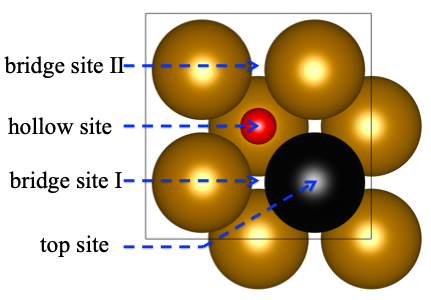
\includegraphics[width=0.65\linewidth]{Chap3/plots/Fig3a.png}}\label{Chap:Mg_H:fig:3a}
  \subfigure[]{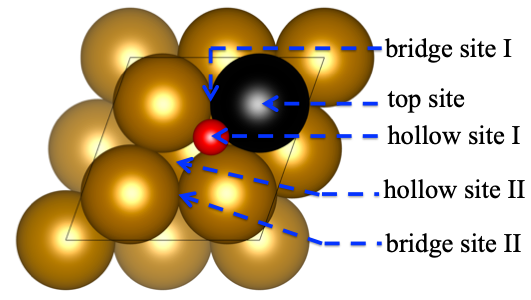
\includegraphics[width=0.75\linewidth]{Chap3/plots/Fig3b.png}}\label{Chap:Mg_H:fig:3b}
\caption[Top-down views of Fe surfaces with substitutional alloying elements and adsorbed H atoms]{Top-down views of Fe (gold) surfaces with substitutional alloying (black) elements and adsorbed H (red) atoms. (a) The (2x2) Fe (100) slab with a generic alloying element substituting a Fe atom in the top surface layer and an adsorbed H atom at the hollow site. (a) The (2x2) Fe (110) slab with a generic alloying element substituting a Fe atom in the top surface layer and an adsorbed H atom at the hollow site I. The concentration of the adsorbed H and the substitutional alloying atom is $\frac{1}{4}$ \ac{ML} for both Fe (100) and Fe (110).}
  \label{Chap:Mg_H:fig3}
\end{figure}
\endgroup